Relativitetsteorien er den gren af fysikken, der beskriver store hastigheder og energier. Der er egentligt to relativitetsteorier; den specielle og den almene.
Som navnet antyder er den specielle relativitetsteori et specialtilfælde af den almene.
Vi vil holde os til den specielle relativitetsteori, da den er både matematisk og konceptuelt simplere.

Relativitetsteorien bygger på to principper, hvor et princip i fysiken er en grundlæggende antagelse.
Det kan virke som om, man bare postulerer, hvad end der er belejligt, men principper er baseret på observationer af naturen og lever kun så længe, som de konklusioner, de fører til, lever op til virkeligheden.
Det første princip vi skal se på er {\em relativitetsprincippet}, der lyder:
%
\begin{quote}
    \emph{Naturens love er ens for alle observatører.}
\end{quote}
%
Relativitetsprincippet er ikke noget nyt. Den første formulering vi kender stammer fra helt tilbage fra 1632.
Dengang beskrev Galileo Galilei, hvordan sommerfugle i kahytten på et skib og røgen fra skibets skorsten ville bevæge sig ens uafhængigt af, hvorvidt skibet er i hvile eller sejler med konstant hastighed. \\
%Dengang beskrev Galileo Galilei hvordan sommerfugle og røg vil bevæge sig ens i alle retninger, både når skibet er i hvile og når det sejler med konstant hastighed.
Den vigtigste pointe her er, at Galileis relativitetsprincip {\em kun} gør sig gældende for konstant hastighed.
Grunden til dette kan findes ved at kigge på Newtons anden lov:
$$
\va F=m\dv[2]{\va x}{t} \: .
$$
Kraften $\va F$ er her defineret ud fra den anden afledte af vores koordinatvektor $\va x$.
Befinder vi os i hvilesystemet, systemet hvor objektet, som vi kigger på, er i hvile, vil de fysiske vekselvirkninger i systemet være årsag til hele kraften. Et system er det koordinatsystem man bruger til at måle placeringer efter. Relativitetsprincippet siger at lige gyldig hvilket koordinatsystem man bruger, så skal fysikkens love beskrive den samme virkelighed -- fysikkens love forudsige de samme resultater af et eksperiment.
Det interessante er, at en observatør, der bevæger sig med konstant hastighed i forhold til dette hvilesystem, vil opleve den samme kraft, siden kraften afhænger af den andenafledede af koordinatvektoren.
Det er således ikke muligt at afgøre, om man er i hvile eller bevæger sig med konstant hastighed.
Vi kalder disse systemer for {\em inertialsystemer}, og de vil være vores fokus i resten af kapitlet.
I ikke-inertielle systemer opstår kræfter, der udelukkende skyldes vores valg af koordinatsystem.
Disse kræfter kaldes inertielle kræfter eller fiktive kræfter.
Det er kræfter som elevatorkræften%\footnote{Det er underordnet at elevatorer sjælendt har konstant acceleration.}
, som man mærker, når man accelererer med konstant acceleration, eller centrifugalkraften, der opleves, når man befinder sig i et roterende system.

Vi betragter nu to systemer $S$ og $S'$, hvor $S'$ bevæger sig med en konstant hastighed $v$ langs $x$-aksen set fra $S$.
Vi ønsker at finde ud af, hvordan man oversætter koordinaterne fra det ene til det andet system.
Til at starte med regner vi klassisk\footnote{Med klassisk mekanik mener man Newtonsk mekanik beskrevet ved Newtons love fremfor kvantemekanik beskrevet ved Schrödingerligningen. Kort sagt betyder ordet ``klassisk'' i fysik at det ikke er ``kvantemekanisk''.}, hvor tiden er ens for alle observatører\footnote{Dette er en vigtig antagelse, da man i speciel relativitetsteori oplever, at længde og tid vil være påvirket af observatørens hastighed relativt til lysets konstante hastighed. Læs mere om dette i afsnittene om tidsforlængelse og længdeforkortelse, henholdsvis afsnit \ref{sec:Tidsforlaengelse} og \ref{sec:Laengdeforkortelse}}:
\begin{subequations}
\begin{equation}
    t'=t \: .
\end{equation}
For at find $x'$, $x$-koordinatet for systemet $S'$, skal vi korrigere for $S'$s bevægelse, hvilket gøres ved
\begin{equation}
    x'=x-vt \: .
\end{equation}
Vinkelret på bevægelsen er der ingen forskel, hvorfor
\begin{align}
    y'&=y \: ,\\
    z'&=z \: .
\end{align}
\label{SR:GalileiTransformationen}
Disse ligninger kaldes samlet for \emph{Galileitransformationerne}, hvilke giver den klassiske beskrivelse af relativitetsteori før Einsteins bidrag hertil.
\end{subequations}

\begin{figure}
    \centering
    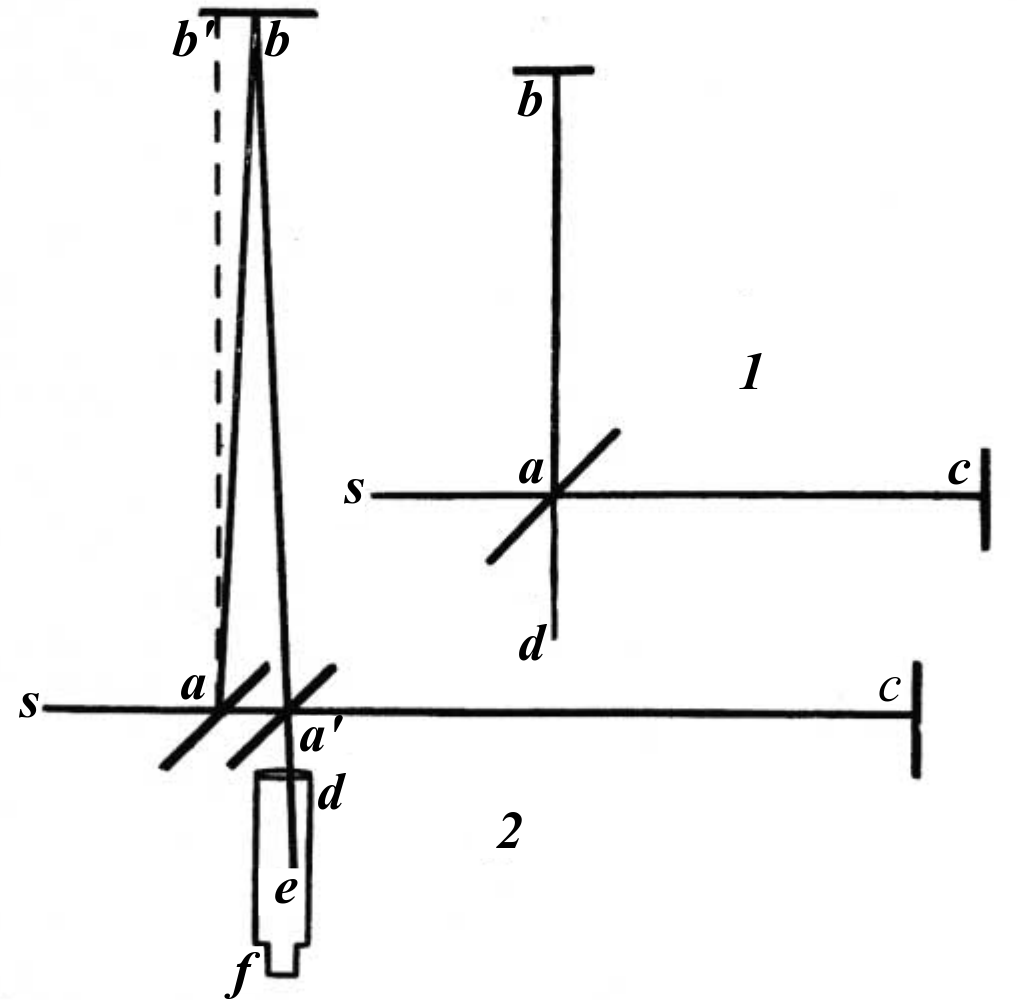
\includegraphics[width=0.5\textwidth]{SR/billeder/MichelsonMorleyInterferometer.png}
    \caption{Michelson og Morley's oprindelige illustration af eksperimentet. Lys udsendes fra $s$ og splittes i to ved $a$. De to stråler sendes tilbage ved $b$ og $c$, hvorefter det igen reflekteres ved $a$ ind imod $d$ hvor det observeres. 1. er opstillingen i hvile i forhold til æteren, og 2. er opstillingen med ætervind langs $sc$-linjen. Som man kan se tilbagelægger lyset send ud imod $b$ her en større afstand, hvilket kan måles som interferens ved $d$. Kilde: \cite{michelsonRelativeMotionEarth1887}.}
    \label{fig:SR:MM}
\end{figure}
%
Det andet centrale princip, som vi har brug for, er, at lysets hastighed er den samme for alle observatører. Eller formuleret lidt anderledes:
\begin{quote}
{\em Lysets hastighed i vakuum er en naturkonstant, og afhænger hverken af kilden eller observatøren.}
\end{quote}
På Einsteins tid var den almindeligt accepterede beskrivelse af lys, at det var elektromagnetiske bølger.
Således mente man, at lyset måtte udbrede sig i et medie ligesom lyd, som udbreder sig som svingninger i luften.
Dette medie havde endda et navn; den lysbærende æter.
Hvis lyset rejser i æteren, vil Jordens bevægelse rund om Solen give ændringer i lysets hastighed, da Jordens relative hastighed ville ændre sig i forhold til det system, hvor æteren var i hvile.
I 1887 forsøgte de amerikanske fysikere Albert A. Michelson og Edward W. Morley at måle denne ætervind. Jorden bevæger sig om Solen med en banehastighed på omkring \SI{30}{km/s}, og lysets hastighed er $\num{10000}$ gange større, så de havde brug for meget fintfølende instrumenter. De sendte en lysstråle ind imod et halvreflekterende spejl (punkt ''a'' på figur \ref{fig:SR:MM}), så den blev splittet i to vinkelrette stråler, der bevægede sig udad, indtil de begge blev reflekteret tilbage af hvert sit spejl (punkterne ''b'' og ''c'' på figur \ref{fig:SR:MM}). Ved det halvreflekterende spejl mødtes strålerne igen, blev sammenlagt og sendt imod en detektor (punkt ''e'' på figur \ref{fig:SR:MM}). Lys er en bølge, så når de to stråler mødes igen kombineres de til en samlet stråle. Hvis armene er præcis lige lange, så vil en bølgetop fra den ene arm møde en bølgetop fra den anden og bølgerne vil da forstærke hinanden. Er den ene arm en smule længere end den anden, så vil en bølgetop fra den ene arm ikke møde en bølgetop fra den anden, og signalet vil ikke blive forstærket ligeså meget. I det tilfælde hvor den ene stråle skal rejse en halv bølgelængde længere end den anden, da vil bølgetoppe fra den ene stråle møde bølgedale fra den anden, og samlet set vil de modvirke hinanden, således at strålen forsvinder. Dette fænomen kaldes interferens og ud fra dette %interferensen på den detekterede stråle 
kunne Michelson og Morley måle forskellen på den tilbagelagte vejlængde for de to dele af strålen. Dette gav dem en utrolig god præcision; faktisk så god en præcision, at Michelson-Morley interferometre bruges i dag, blandt andet i LIGO\footnote{Tyngdebølgeobservatoriet, der i 2015 bekræftede at tyngdebølger eksisterer.}, hvor netop præcision er påkrævet.
På trods af deres gode opsætning fandt Michelson og Morley ingen spor af ætervind.
I dag ved vi, at dette resultat skyldes, at æteren ikke eksisterer.
Æteren blev dog ikke aflivet af Michelson og Morley, og deres resultat blev først forklaret tilfredsstillende i 1905, da Einstein indså, at lys ikke krævede et udbredelsesmedie\footnote{Den fundementale forskel imellem lys og andre bølger, såsom lyd, er at lys er elektriske og magnetiske felter, der giver ophav til hinanden, og ikke forstyrelser i et medie.}.